\subsection{Pantalla: Géstionar Usuarios.}
%IUGestPerfiles
\subsubsection{Objetivo}
	El mapa de navegación se muestra en la Figura~\ref{fig:mapaNavegacionCU1}

   \begin{figure}[hbpt!]
 		\centering
 			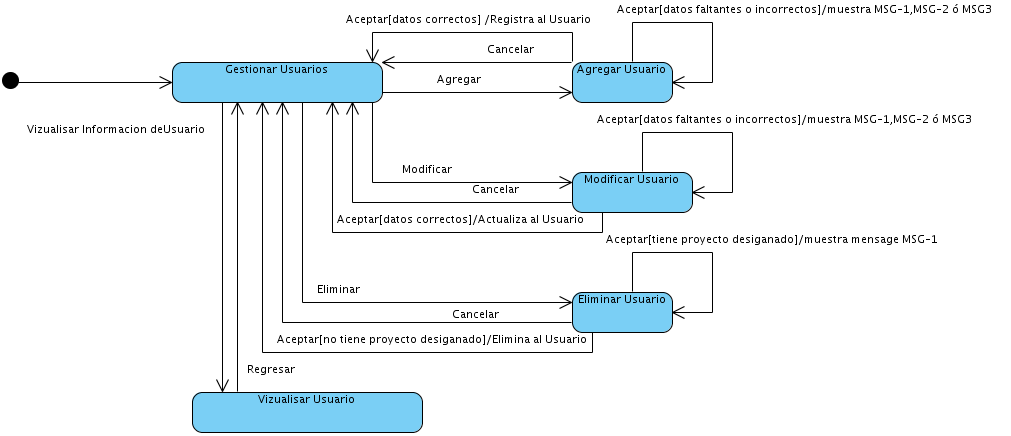
\includegraphics[width=0.8\textwidth]{images/CU1/NavegacionUsuarios.png}
 		\caption{Mapa de navegacion para el CU 1 Gestion de Usuarios.}
		\label{fig:mapaNavegacionCU1}
 	\end{figure}

\subsubsection{Objetivo}
Mostrar el menú para buscar, agregar, modificar o eliminar datos de un usuario y acceso a otras funciones.
Figura~\ref{IUGestUsuarios}

\IUfig[0.6]{CU1/GestionUsuarios.png}{IUGestUsuarios}{Pantalla: Géstionar Usuarios.}
%\IUfig[0.8]{cu1/GestionUsuariosSinDatos.png}{IUGestUsuariosSinDatos}{Pantalla: Géstionar Usuarios sin usuarios registrados.}
%IUPCAdminTdU es el identificador par ala referencia
\subsubsection{Salidas}
Se muestra la lista de los Usuarios registrados, ordenados por nombre y mostrando algunos de sus datos como:
\begin{itemize}
 \item Nombre
 \item Apellido Paterno
 \item Apellido Materno
 \item Perfil
 \item Área
\end{itemize}

\subsubsection{Controles}
\begin{itemize}
 \item \IUbutton{Flecha derecha} Muestra los siguientes n ejes temáticos.
 \item \IUbutton{Flecha izquierda} Muestra los n ejes temáticos anteriores.
\end{itemize}

\subsubsection{Comandos}
\begin{itemize}
 \item \IUbutton{Agregar Nuevo Usuario} Muestra la pantalla \IUref{IUAgregarUsuario}{Agregar Usuario}.
 \item \IUbutton{
\includegraphics[scale=0.1]{images/icons/editar.png}} Permite realizar modificaciones a un Usuario selecionado.\IUref{IUModificarUsuario}{Modificar Usuario}.
 \item \IUbutton{
\includegraphics[scale=0.1]{images/icons/eliminar.png}} Elimina el registro de un Usuario del sistema siempre y cuando no tenga proyectos asociados.\IUref{IUEliminarUsuario}{Eliminar Usuario.}
 %\item \IUbutton{
\includegraphics[scale=0.1]{images/icons/ver.png}} Muestra los datos completos del Usuario. \IUref{IUVisualizarUsuario}{Visualizar Usuario.}

\end{itemize}


